\documentclass[12pt,a4paper]{article}

\usepackage[utf8]{inputenc}
\usepackage{amsmath,amssymb,amsfonts}
\usepackage{graphicx}
\usepackage{hyperref}
\usepackage{geometry}
\usepackage{fancyhdr}
\usepackage{listings}
\usepackage{xcolor}
\usepackage{booktabs}
\usepackage{pgfplots}
\usepackage{pgfplotstable}
\usepackage{float}
\usepackage{url}

\geometry{margin=1in}

\hypersetup{
    colorlinks=true,
    linkcolor=blue,
    filecolor=magenta,
    urlcolor=cyan,
    pdftitle={ML Experiment Triage Environment - Technical Documentation},
    pdfpagemode=FullScreen,
}

\lstset{
    backgroundcolor=\color{gray!10},
    basicstyle=\ttfamily\small,
    breaklines=true,
    frame=single,
    captionpos=b,
    numbers=left,
    numberstyle=\tiny\color{gray},
}

\pagestyle{fancy}
\fancyhf{}
\rhead{\thepage}
\lhead{ML Experiment Triage Environment}
\rfoot{Technical Documentation}

\title{\textbf{ML Experiment Triage Environment}\\\large A Reinforcement Learning Environment for ML Experiment Analysis}

\author{Charan Sai Ponnada\\Scaler School of Technology}

\date{\today}

\begin{document}

\maketitle

\begin{abstract}
	This document provides comprehensive technical documentation for the ML Experiment Triage Environment, an OpenEnv-compliant reinforcement learning environment designed for automating the analysis and triage of machine learning experiment results. The system enables AI agents to identify best-performing experiments, detect overfitting, and suggest optimal hyperparameter configurations through a structured action-space interface. This environment was developed for the Meta PyTorch Hackathon and implements state-of-the-art practices in RL environment design.
\end{abstract}

\newpage

\tableofcontents

\newpage

\section{Introduction}

\subsection{Background and Motivation}

Machine learning development involves running numerous experiments with varying hyperparameters, architectures, and training strategies. Manually reviewing each experiment's results to identify the best configurations is time-consuming and error-prone. The ML Experiment Triage Environment addresses this challenge by simulating an RL environment where an AI agent learns to efficiently triage experiment results.

\subsection{Problem Statement}

Given a set of ML experiment results, the agent must:
\begin{itemize}
	\item \textbf{Identify the best experiment} among multiple runs
	\item \textbf{Detect overfitting} patterns in training metrics
	\item \textbf{Suggest next configurations} based on observed patterns
	\item \textbf{Compare experiments} and analyze performance trade-offs
	\item \textbf{Debug failed runs} and diagnose root causes
\end{itemize}

\subsection{Contributions}

The main contributions of this work are:
\begin{enumerate}
	\item An OpenEnv-compliant RL environment with structured action and observation spaces
	\item Five distinct tasks covering various ML experiment analysis scenarios
	\item A Gradio-based web interface for human-in-the-loop evaluation
	\item Docker containerization for easy deployment and evaluation
	\item Integration with LiteLLM proxy for standardized LLM inference
\end{enumerate}

\section{System Architecture}

\subsection{Overview}

The system consists of three main components:

\begin{figure}[H]
	\centering
	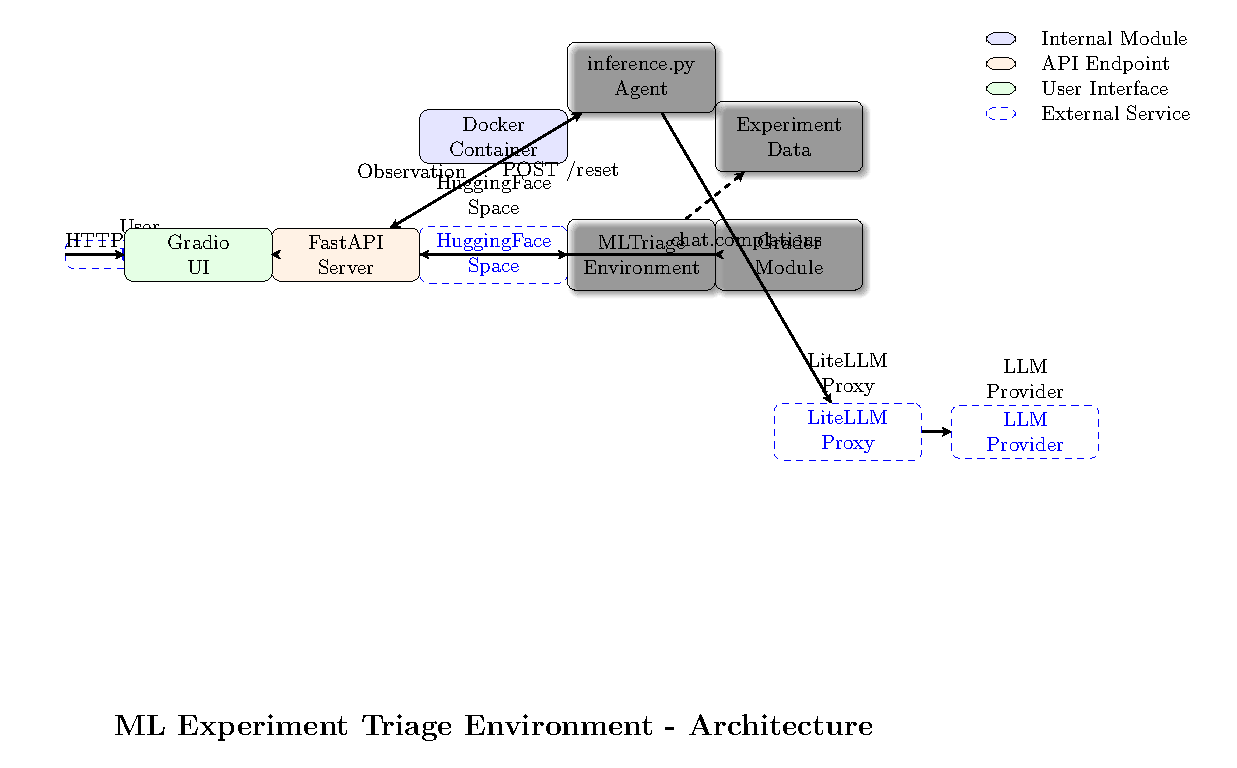
\includegraphics[width=0.8\textwidth]{architecture.pdf}
	\caption{System Architecture Diagram}
	\label{fig:architecture}
\end{figure}

\subsection{Component Description}

\subsubsection{Environment Server}
The environment server (\texttt{server/}) implements the OpenEnv interface:
\begin{itemize}
	\item \texttt{ml\_triage\_environment.py}: Core environment implementation
	\item \texttt{app.py}: FastAPI application with OpenEnv integration
	\item Handles reset, step, and state operations
\end{itemize}

\subsubsection{Web Interface}
The web interface (\texttt{app/}) provides a Gradio-based UI:
\begin{itemize}
	\item \texttt{main.py}: FastAPI server with static file serving
	\item \texttt{env.py}: Custom environment with LLM integration
	\item \texttt{templates/index.html}: Interactive Gradio interface
	\item Real-time experiment visualization and action feedback
\end{itemize}

\subsubsection{Inference Pipeline}
The inference pipeline (\texttt{inference.py}) runs autonomous evaluation:
\begin{itemize}
	\item Connects to environment via REST API
	\item Uses LLM for action decision-making
	\item Outputs structured logs for evaluation
\end{itemize}

\section{Environment Specification}

\subsection{Observation Space}

The observation space is a structured dictionary containing:

\begin{table}[H]
	\centering
	\caption{Observation Space Fields}
	\begin{tabular}{@{}lp{10cm}@{}}
		\toprule
		\textbf{Field}             & \textbf{Description}               \\
		\midrule
		\texttt{experiments}       & List of ExperimentRecord objects   \\
		\texttt{current\_step}     & Current step number (0-indexed)    \\
		\texttt{max\_steps}        & Maximum allowed steps for the task \\
		\texttt{task\_description} & Natural language task description  \\
		\texttt{feedback}          & Feedback from the previous action  \\
		\texttt{serialized\_state} & Additional state information       \\
		\bottomrule
	\end{tabular}
\end{table}

\subsection{Action Space}

The action space consists of four discrete actions:

\begin{enumerate}
	\item \texttt{investigate(exp\_id)}: Examine an experiment's details
	\item \texttt{discard(exp\_id)}: Mark an experiment as not worth keeping
	\item \texttt{suggest(suggestion)}: Propose next hyperparameter configuration
	\item \texttt{summarize(summary)}: Provide final answer and end episode
	\item \texttt{compare(comparison)}: Compare two experiments (Tasks 4)
	\item \texttt{diagnose(diagnosis)}: Diagnose a failed run (Task 5)
\end{enumerate}

\subsection{Experiment Record Schema}

\begin{lstlisting}[language=Python, caption={ExperimentRecord Model}]
@dataclass
class ExperimentRecord:
    exp_id: str           # Unique experiment identifier
    model_name: str        # Model architecture name
    learning_rate: float   # Learning rate
    epochs: int           # Number of training epochs
    train_acc: float      # Training accuracy
    val_acc: float       # Validation accuracy
    train_loss: float     # Training loss
    val_loss: float      # Validation loss
    notes: str           # Additional notes
    status: str          # Status: pending, investigated, discarded
\end{lstlisting}

\section{Task Specifications}

\subsection{Task 1: Find Best Experiment}

\textbf{Difficulty:} Easy

\textbf{Objective:} Identify the single best performing experiment from a set of 8 runs.

\textbf{Grading Criteria:}
\begin{itemize}
	\item Correctly identify exp\_004 as the best experiment: 0.9999
	\item Investigate exp\_004 without summarizing: 0.5
	\item No correct identification: 0.0001
\end{itemize}

\textbf{Action Pattern:} The agent should investigate multiple experiments and use \texttt{summarize} with the correct exp\_id.

\subsection{Task 2: Identify Overfitting}

\textbf{Difficulty:} Medium

\textbf{Objective:} Detect and discard all 3 overfitting experiments.

\textbf{Overfitting Definition:} An experiment is overfitting if:
\begin{equation}
	\text{train\_acc} > 0.97 \quad \text{and} \quad \text{val\_acc} < 0.75
\end{equation}

\textbf{Grading Formula:}
\begin{equation}
	\text{score} = \frac{\text{correct\_discards}}{3} - 0.1 \times \text{wrong\_discards}
\end{equation}

\textbf{Target Experiments:} exp\_002, exp\_006, exp\_009

\subsection{Task 3: Suggest Next Experiment}

\textbf{Difficulty:} Hard

\textbf{Objective:} Based on incomplete experiment results, suggest the next hyperparameter configuration.

\textbf{Grading Criteria:}
\begin{itemize}
	\item All 3 fields correct (lr=0.001, epochs=50, model=resnet50): 0.9999
	\item 2 fields correct: 0.6
	\item 1 field correct: 0.3
	\item No fields correct: 0.0001
\end{itemize}

\subsection{Task 4: Compare Experiments}

\textbf{Difficulty:} Medium

\textbf{Objective:} Compare two experiments and analyze performance trade-offs.

\textbf{Scoring Keywords:}
\begin{itemize}
	\item exp\_004 mentioned: +0.4
	\item validation metrics analyzed: +0.2
	\item generalization discussed: +0.2
	\item trade-off analysis: +0.2
\end{itemize}

\subsection{Task 5: Debug Failed Run}

\textbf{Difficulty:} Hard

\textbf{Objective:} Diagnose the root cause of a failed experiment run.

\textbf{Known Failure Modes:}
\begin{itemize}
	\item exp\_005: Learning rate issues (high)
	\item exp\_008: Memory/OOM issues
	\item exp\_003: Training plateau issues
\end{itemize}

\section{Reward System}

\subsection{Reward Structure}

The environment uses dense rewards for step-by-step feedback:

\begin{table}[H]
	\centering
	\caption{Reward Values by Action}
	\begin{tabular}{@{}lr@{}}
		\toprule
		\textbf{Action}               & \textbf{Reward} \\
		\midrule
		Successful investigate        & +0.1            \\
		Correct discard (overfitting) & +0.05           \\
		Incorrect discard             & -0.1            \\
		Invalid action                & -0.05           \\
		Episode completion            & 0.0 to 1.0      \\
		\bottomrule
	\end{tabular}
\end{table}

\subsection{Final Score Calculation}

The final score is clamped to ensure strict bounds:
\begin{equation}
	\text{final\_score} = \max(10^{-9}, \min(1 - 10^{-9}, \text{sum}(\text{rewards})))
\end{equation}

\section{Implementation Details}

\subsection{Server Implementation}

\begin{lstlisting}[language=Python, caption={Environment Factory}]
def create_env():
    return MLTriageEnvironment()

app = create_app(
    create_env,
    MLTriageAction,
    MLTriageObservation,
    env_name="ml-experiment-triage"
)
\end{lstlisting}

\subsection{Grader Implementation}

\begin{lstlisting}[language=Python, caption={Task Grading Function}]
def grade_task_1(experiments, episode_history, summary):
    investigated_exp_ids = set()
    for step in episode_history:
        if step["action"]["action_type"] == "investigate":
            investigated_exp_ids.add(step["action"]["exp_id"])
    
    if summary and "exp_004" in summary:
        return _clamp_strict(0.9999)
    
    if "exp_004" in investigated_exp_ids:
        return 0.5
    
    return _clamp_strict(0.0001)
\end{lstlisting}

\subsection{Inference Pipeline}

\begin{lstlisting}[language=Python, caption={LLM Action Generation}]
def get_action(obs_text: str, history: list) -> dict:
    messages = [{"role": "system", "content": SYSTEM_PROMPT}]
    for h in history[-6:]:
        messages.append({"role": "user", "content": h["obs"]})
        messages.append({"role": "assistant", "content": h["action"]})
    messages.append({"role": "user", "content": obs_text})
    
    resp = client.chat.completions.create(
        model=MODEL_NAME,
        messages=messages,
        max_tokens=MAX_TOKENS,
        temperature=TEMPERATURE,
    )
    return json.loads(resp.choices[0].message.content)
\end{lstlisting}

\section{Deployment}

\subsection{Docker Container}

The application is containerized using Docker:

\begin{lstlisting}[caption={Dockerfile}]
FROM python:3.11-slim

WORKDIR /app
RUN pip install uv
RUN uv pip install --system fastapi openai openenv-core \
    pydantic pyyaml uvicorn jinja2 python-multipart requests

COPY server/ ./server/
COPY app/ ./app/
COPY models.py ./
COPY inference.py ./

EXPOSE 7860
CMD ["python", "-c", "from app.main import app; \
    import uvicorn; uvicorn.run(app, host='0.0.0.0', port=7860)"]
\end{lstlisting}

\subsection{HuggingFace Space}

The environment is deployed as a HuggingFace Space:

\begin{itemize}
	\item SDK: Docker
	\item Port: 7860
	\item Hardware: CPU (default)
	\item Repository: \url{https://huggingface.co/spaces/Charansaiponnada/ml-experiment-triage-env}
\end{itemize}

\section{API Reference}

\subsection{REST Endpoints}

\subsubsection{POST /reset}

Reset the environment for a new episode.

\begin{lstlisting}[caption={Reset Request}]
POST /reset
Content-Type: application/json

{"task_id": 1}
\end{lstlisting}

Response:
\begin{lstlisting}[caption={Reset Response}]
{
    "observation": {...},
    "reward": null,
    "done": false
}
\end{lstlisting}

\subsubsection{POST /step}

Execute an action in the environment.

\begin{lstlisting}[caption={Step Request}]
POST /step
Content-Type: application/json

{"action": {"action_type": "investigate", "exp_id": "exp_001"}}
\end{lstlisting}

\subsubsection{GET /health}

Health check endpoint.

\begin{lstlisting}[caption={Health Response}]
{"status": "ok"}
\end{lstlisting}

\section{Evaluation Metrics}

\subsection{Score Calculation}

Each task returns a score in the range $(0, 1)$:

\begin{itemize}
	\item Scores of exactly 0.0 or 1.0 are rejected
	\item Epsilon padding ($10^{-9}$) ensures strict bounds
	\item Final submission score is the average across all tasks
\end{itemize}

\subsection{Success Criteria}

A submission is considered successful if:
\begin{enumerate}
	\item Docker container builds successfully
	\item inference.py executes without errors
	\item Output parsing validates correctly
	\item All task scores are in $(0, 1)$
	\item LLM calls go through the provided LiteLLM proxy
\end{enumerate}

\section{Future Work}

\subsection{Potential Improvements}

\begin{itemize}
	\item \textbf{Multi-agent support}: Extend to allow multiple agents to collaborate
	\item \textbf{Custom datasets}: Allow users to upload their own experiment data
	\item \textbf{Advanced metrics}: Add more sophisticated evaluation metrics
	\item \textbf{Transfer learning}: Pre-train agents on synthetic data
	\item \textbf{Human feedback integration}: Allow human correction during episodes
\end{itemize}

\section{Conclusion}

The ML Experiment Triage Environment provides a robust framework for training and evaluating AI agents in the task of ML experiment analysis. Through its structured action space, diverse task set, and comprehensive evaluation system, it enables researchers to develop and benchmark intelligent agents for automating the tedious process of experiment triage.

The environment's compliance with the OpenEnv standard ensures compatibility with the broader ecosystem of RL environments, while its Docker and HuggingFace deployment options make it accessible for both local development and cloud-based evaluation.

\newpage

\section*{Appendices}

\subsection{Appendix A: File Structure}

\begin{verbatim}
ml-experiment-triage-env/
├── app/
│   ├── main.py           # FastAPI web server
│   ├── env.py            # Custom environment with LLM
│   ├── models.py         # Pydantic models
│   ├── tasks.py          # Task definitions and graders
│   ├── data.py           # Experiment data generation
│   └── templates/
│       └── index.html    # Web interface
├── server/
│   ├── app.py            # OpenEnv integration
│   └── ml_triage_environment.py  # Core environment
├── inference.py          # Autonomous evaluation script
├── models.py             # Shared Pydantic models
├── Dockerfile            # Container definition
├── openenv.yaml         # Environment specification
└── README.md            # Project documentation
\end{verbatim}

\subsection{Appendix B: Environment Variables}

\begin{table}[H]
	\centering
	\caption{Environment Variables}
	\begin{tabular}{@{}lll@{}}
		\toprule
		\textbf{Variable} & \textbf{Default}          & \textbf{Description} \\
		\midrule
		API\_BASE\_URL    & router.huggingface.co/v1  & LLM endpoint         \\
		API\_KEY          & -                         & Authentication key   \\
		HF\_TOKEN         & -                         & HuggingFace token    \\
		MODEL\_NAME       & Qwen/Qwen2.5-72B-Instruct & LLM model            \\
		ENV\_BASE\_URL    & http://localhost:7860     & Environment URL      \\
		\bottomrule
	\end{tabular}
\end{table}

\subsection{Appendix C: Acknowledgments}

This project was developed for the Meta PyTorch Hackathon x Scaler School of Technology, Round 1. We acknowledge the OpenEnv team for providing the environment framework and HuggingFace for hosting infrastructure.

\newpage

\section*{References}

\begin{enumerate}
	\item OpenEnv Core Documentation. \url{https://github.com/openenv/core}
	\item OpenAI API Reference. \url{https://platform.openai.com/docs/api-reference}
	\item LiteLLM Documentation. \url{https://docs.litellm.ai/}
	\item HuggingFace Spaces. \url{https://huggingface.co/docs/hub/spaces}
	\item Gradio Documentation. \url{https://gradio.app/docs/}
\end{enumerate}

\end{document}
